%%%%%%%%%%%%%%%%%%%%%%%%%%%%%%%%%%%%%%%%%%%%%%%%%%%%%%%%%%
%%
%% MARK: Title
%%
%%%%%%%%%%%%%%%%%%%%%%%%%%%%%%%%%%%%%%%%%%%%%%%%%%%%%%%%%%

\chapter*{\S B26. The Wire Plane and its Topology}
\setcounter{footnote}{0}

%%%%%%%%%%%%%%%%%%%%%%%%%%%%%%%%%%%%%%%%%%%%%%%%%%%%%%%%%%
%%
%% MARK: Abstract
%%
%%%%%%%%%%%%%%%%%%%%%%%%%%%%%%%%%%%%%%%%%%%%%%%%%%%%%%%%%%

\begin{abstract}
  We introduce the \emph{Wire Plane} $\cW$,
  a diffeological space whose underlying set is $\RR^2$
  but whose smooth structure is defined by plots that factor locally through smooth curves.
  We prove that the D-topology of $\cW$ coincides with the standard Euclidean topology,
  yet the diffeological dimension of $\cW$ is $1$,
  not $2$.
  This is the first step in exhibiting the \emph{Boman Paradox}:
  two diffeological spaces with identical topology and identical abstract diffeomorphism groups
  that are nevertheless geometrically distinct.
\end{abstract}

%%%%%%%%%%%%%%%%%%%%%%%%%%%%%%%%%%%%%%%%%%%%%%%%%%%%%%%%%%
%%
%% MARK: Introduction
%%
%%%%%%%%%%%%%%%%%%%%%%%%%%%%%%%%%%%%%%%%%%%%%%%%%%%%%%%%%%

What is a geometry?
A classical answer,
descending from Klein's Erlangen Program,
is that a geometry is determined by a space together with a group of symmetries acting upon it.
In the context of differential geometry,
Jean-Marie Souriau pushed this idea to its extreme,
claiming that ``le groupe est la géométrie'' \cite{Sou84}.
To realize this program,
he introduced \emph{difféologies} (now diffeology) to give a smooth structure to infinite-dimensional groups of diffeomorphisms.

The present work,
and the following one,
reveal a limit to this radical perspective.
We construct a diffeological space,
the \emph{Wire Plane} $\cW$,
which is indistinguishable from the standard Euclidean plane $\RR^2$ from the viewpoints of classical topology and abstract group theory,
yet is geometrically distinct:
its diffeological dimension is $1$, not $2$,
and its group of diffeomorphisms,
while identical as a set to $\Diff(\RR^2)$,
carries a strictly finer diffeology.

This chapter focuses on the topological identity.
We define $\cW$,
compute its D-topology,
and establish its dimension.
The next chapter (B27) will analyze its group of diffeomorphisms and complete the paradox.

%%%%%%%%%%%%%%%%%%%%%%%%%%%%%%%%%%%%%%%%%%%%%%%%%%%%%%%%%%
%%
%% MARK: Definition of the Wire Plane
%%
%%%%%%%%%%%%%%%%%%%%%%%%%%%%%%%%%%%%%%%%%%%%%%%%%%%%%%%%%%
\section{Definition of the Wire Plane}

Let us recall the definition of a diffeological space.
A diffeology on a set $X$ is a collection of maps $P: U \to X$,
called \emph{plots},
where $U$ is an open subset of some $\RR^n$,
satisfying three axioms:
covering (constant maps are plots),
locality (a map is a plot if it is locally a plot),
and smooth compatibility (plots compose with smooth maps).

\begin{figure}[th]
  \centerline{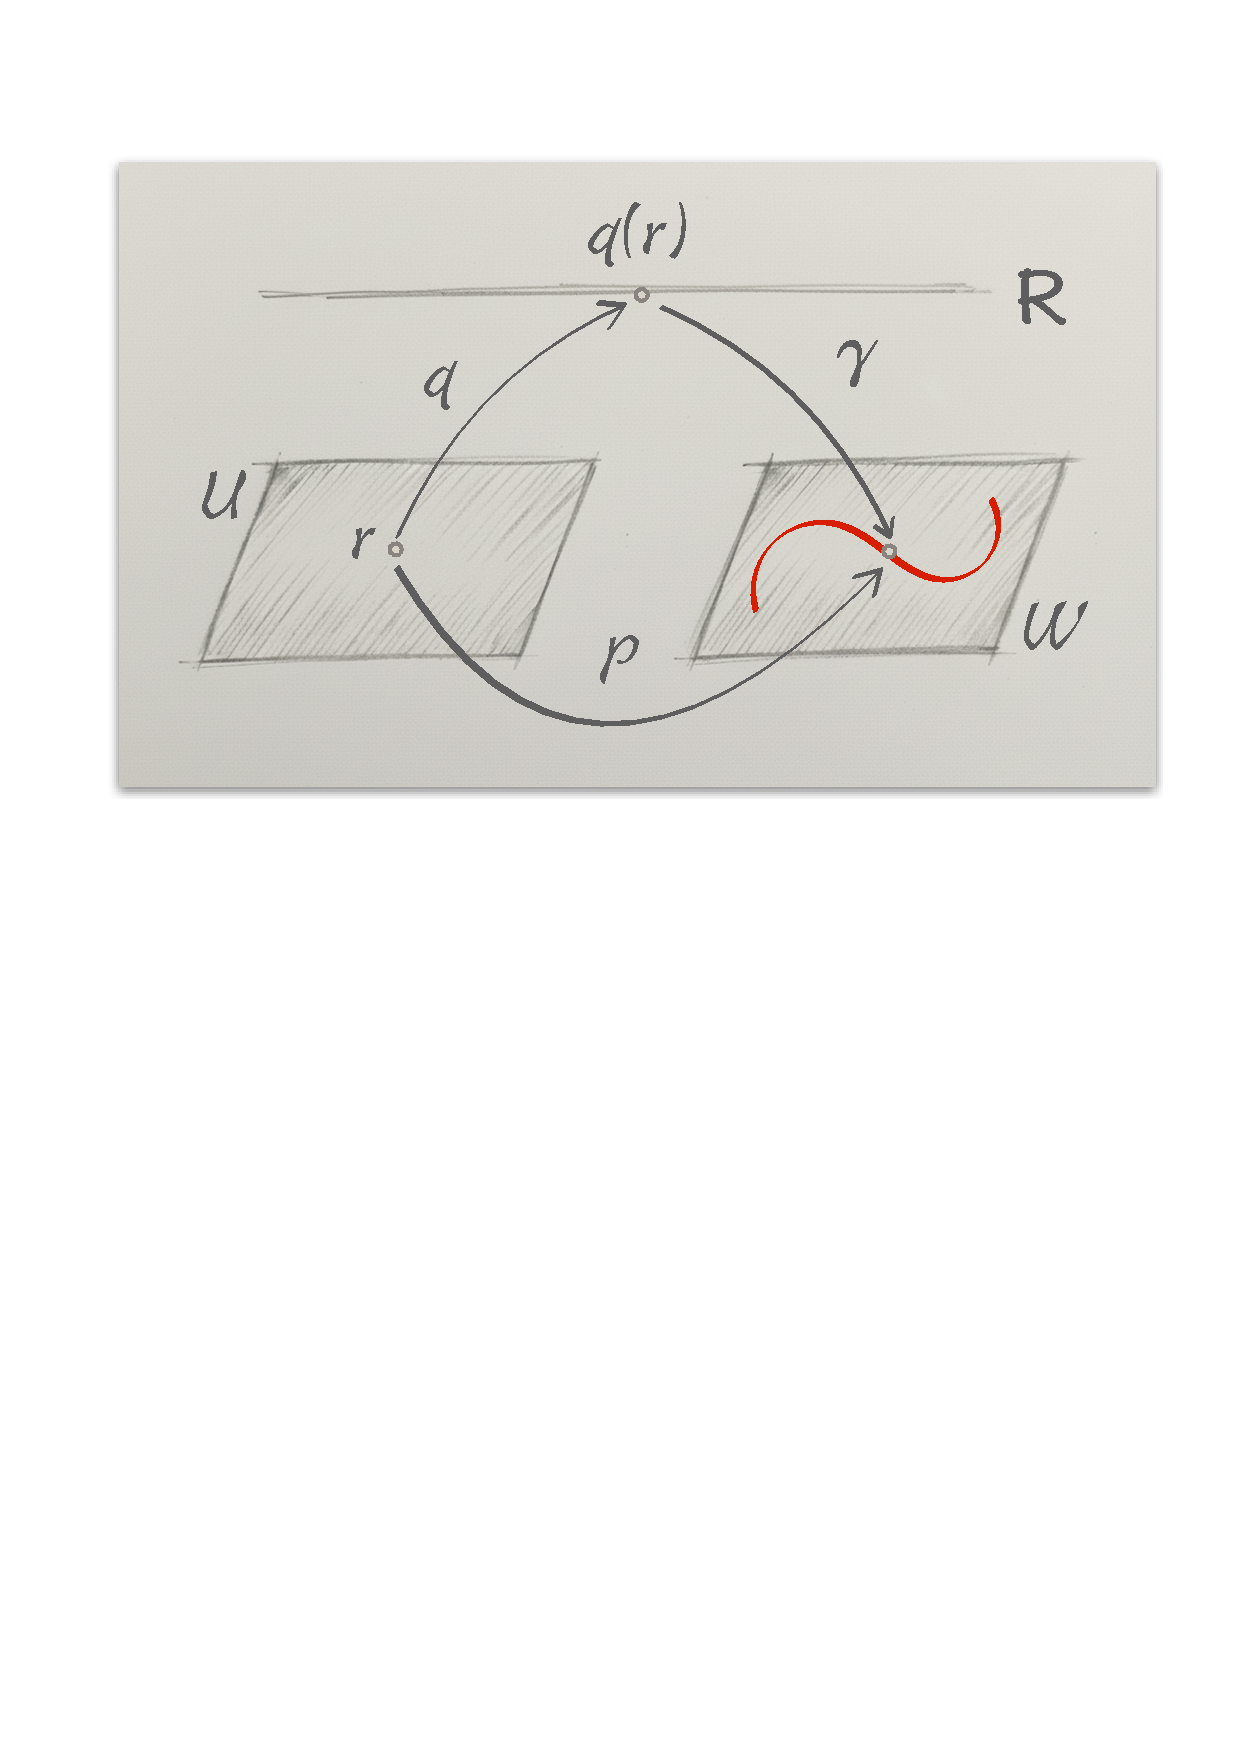
\includegraphics[width=0.5\textwidth]{Figures/Wire-plot.pdf}}
  \vspace{-0ex}
  \caption{Every plot of $\cW$ factors locally as $\gamma \circ q$,
  where $\gamma$ is a smooth curve and $q$ is a smooth real-valued function.}
  \label{fig:wire-plot}
\end{figure}

\begin{Article}{The Wire Diffeology}{}
  Let $\cW$ be the set $\RR^2$.
  A parametrization $P: U \to \RR^2$ (with $U \subset \RR^n$ open) is a \emph{plot} of $\cW$ if and only if,
  for every $u \in U$,
  there exists an open neighborhood $V \subset U$ of $u$,
  a smooth curve $\gamma: \RR \to \RR^2$,
  and a smooth function $q: V \to \RR$ such that
  $$%
    P|_V = \gamma \circ q.
    $$%
  In other words,
  $P$ factors locally through a smooth curve.
\end{Article}

\begin{Article}{Example 1.}{}
  The map $P(u,v) = (\sin(u^2+v^2), \cos(u^2+v^2))$ is a plot of $\cW$,
  since it factors as $\gamma(t) = (\sin t, \cos t)$ with $q(u,v) = u^2+v^2$.
\end{Article}

\begin{Article}{Example 2.}{}
  The identity map $\Id(u,v) = (u,v)$ is \emph{not} a plot of $\cW$.
  It cannot be factored locally through a smooth curve,
  as its image contains an open subset of $\RR^2$,
  which has dimension $2$,
  while the image of any factorization $\gamma \circ q$ is contained in the $1$-dimensional image of the curve $\gamma$.
\end{Article}

These two examples already indicate that $\cW$ and the standard plane $\RR^2$ (with its usual diffeology) are different:
the identity map is a plot of $\RR^2$ but not of $\cW$.

%%%%%%%%%%%%%%%%%%%%%%%%%%%%%%%%%%%%%%%%%%%%%%%%%%%%%%%%%%
%%
%% MARK: Dimension of the Wire Plane
%%
%%%%%%%%%%%%%%%%%%%%%%%%%%%%%%%%%%%%%%%%%%%%%%%%%%%%%%%%%%
\section{Dimension of the Wire Plane}

In diffeology,
the dimension of a space is defined by a minimax principle:
it is the infimum over all generating families of plots of the supremum of the dimensions of their domains,
provided the space is not discrete \cite[\textsection\,1.78]{PIZ13}.

\begin{Article}{The dimension of the Wire Plane}{}
  The diffeological dimension of $\cW$ is $1$:
  $$%
    \dim(\cW) = 1.
    $$%
  In contrast,
  the standard plane $\RR^2$ has dimension $2$,
  since the identity plot $\Id: \RR^2 \to \RR^2$ has domain dimension $2$ and generates the diffeology.
  
  Thus,
  $\cW$ and $\RR^2$ have different diffeological dimensions
  despite having the same underlying set.
  This is the first geometric divergence.
\end{Article}

\begin{proof}
  Indeed,
  by definition,
  every plot of $\cW$ factors locally through a smooth curve $\gamma: \RR \to \RR^2$.
  The domain of a curve is $1$-dimensional.
  Hence the dimension of $\cW$ is at most $1$.
  The space $\cW$ is not discrete
  (for example,
  the plot $t \mapsto (t,0)$ is not locally constant),
  therefore its dimension is exactly $1$.
\end{proof}

%%%%%%%%%%%%%%%%%%%%%%%%%%%%%%%%%%%%%%%%%%%%%%%%%%%%%%%%%%
%%
%% MARK: The D-Topology of the Wire Plane
%%
%%%%%%%%%%%%%%%%%%%%%%%%%%%%%%%%%%%%%%%%%%%%%%%%%%%%%%%%%%
\section{The D-Topology of the Wire Plane}

Every diffeological space carries a natural topology,
called the \emph{D-topology},
which is the finest topology making all plots continuous \cite[\textsection\,2.8]{PIZ13}.
A subset $O \subset X$ is D-open if and only if $P^{-1}(O)$ is open in $\Domain(P)$ for every plot $P$.

Let $\tau_{\text{std}}$ denote the standard Euclidean topology on $\RR^2$,
and $\tau_{\cW}$ denote the D-topology of $\cW$.
We shall see in this section that,
paradoxically,
these two topologies $\tau_{\text{std}}$ and $\tau_{\cW}$ coincide.

\begin{Article}{The D-Topology of the Wire Plane}
  \label{prop:topology-identity}
  The D-topology of the Wire Plane coincides with the standard Euclidean topology:
  $$%
    \tau_{\cW} = \tau_{\text{std}}.
    $$%
  The D-topology of $\cW$ is Hausdorff,
  second countable,
  and locally Euclidean of dimension $2$,
  yet the diffeological dimension of $\cW$ is $1$.
  
  Thus,
  from a purely topological perspective,
  $\cW$ is indistinguishable from $\RR^2$.
  The difference lies entirely in the smooth structure.
\end{Article}

\begin{proof}
  we prove the two inclusions separately.
  
  \textbf{1.} $\tau_{\text{std}} \subseteq \tau_{\cW}$.
  
  Let $O \subset \RR^2$ be Euclidean open.
  For any plot $P: U \to \cW$,
  $P$ is locally of the form $\gamma \circ q$,
  where $\gamma$ is smooth and $q$ is smooth.
  Since $\gamma$ is continuous with respect to the Euclidean topology,
  $(\gamma \circ q)^{-1}(O) = q^{-1}(\gamma^{-1}(O))$ is open in $U$.
  Hence $O$ is D-open.
  Thus every Euclidean open set is D-open.
  
  \textbf{2.} $\tau_{\cW} \subseteq \tau_{\text{std}}$.
  
  We prove the contrapositive.
  Assume $O \subset \RR^2$ is a D-open subset that is not Euclidean open.
  Then there exists a point $x \in O$ and a sequence $\{x_n\}$ in the complement $\RR^2 \setminus O$ such that $x_n \to x$ in the Euclidean norm.
  By Lemma \ref{lem:smooth-curve}, there exists a smooth curve $\gamma: \RR \to \RR^2$ and a decreasing sequence $t_k \to 0^+$ such that $\gamma(t_k) = x_{n_k}$ for a subsequence $\{x_{n_k}\}$ of $\{x_n\}$, and $\gamma(0)=x$.
  
  Since $\gamma$ is a smooth curve,
  it is a plot of $\cW$.
  If $O$ were D-open,
  then $\gamma^{-1}(O)$ would be open in $\RR$.
  But $0 \in \gamma^{-1}(O)$ (because $\gamma(0)=x \in O$),
  while every neighborhood of $0$ contains points $t_k$ for which $\gamma(t_k)=x_{n_k} \notin O$.
  This is a contradiction.
  Therefore $O$ must be Euclidean open.
  
  The two inclusions together give $\tau_{\cW} = \tau_{\text{std}}$.
\end{proof}

%%%%%%%%%%%%%%%%%%%%%%%%%%%%%%%%%%%%%%%%%%%%%%%%%%%%%%%%%%
%%
%% MARK: Technical Lemma
%%
%%%%%%%%%%%%%%%%%%%%%%%%%%%%%%%%%%%%%%%%%%%%%%%%%%%%%%%%%%
\section{Smooth curve through a convergent sequence}

The proof of Proposition \ref{prop:topology-identity} relies heavily on the following lemma:
given a convergent sequence of points in $\RR^2$ and its limit, there exists a smooth curve that passes through a subsequence of these points and through the limit.
Explicitly:

\begin{Article}{Smooth curve through a convergent sequence}{}
  \label{lem:smooth-curve}
  Let $\{x_n\}$ be a sequence in $\RR^2$ converging to $x$.
  Then there exists a smooth curve $\gamma: \RR \to \RR^2$,
  a decreasing sequence $t_k \to 0^+$,
  and a subsequence $\{x_{n_k}\}$ of $\{x_n\}$
  such that $\gamma(t_k) = x_{n_k}$ for all $k$,
  and $\gamma(0)=x$.
\end{Article}

\begin{proof}
  We construct $\gamma$ explicitly.
  
  \textbf{Step 1. Setup.}
  Fix the sequence of times $t_k = 1/k$.
  Note that $t_1 > t_2 > t_3 > \cdots$ and $t_k \to 0^+$.
  The interval lengths are
  $$%
    \Delta t_k := t_k - t_{k+1} = \frac{1}{k(k+1)}.
    $$%
  Observe that $0 < \Delta t_{k+1} < \Delta t_k < 1$ for all $k \ge 1$.
  
  Let $\lambda: \RR \to [0,1]$ be a fixed smooth step function with the following properties:
  \begin{itemize}
    \item $\lambda(s)=0$ for $s \le 0$,
    \item $\lambda(s)=1$ for $s \ge 1$,
    \item $\lambda$ is strictly increasing on $[0,1]$.
  \end{itemize}
  Because $\lambda$ is smooth and constant outside $(0,1)$,
  all its derivatives are bounded.
  For each integer $m \ge 1$, define
  $$%
    C_m = \max_{s \in [0,1]} |\lambda^{(m)}(s)| < \infty.
    $$%
  
  \textbf{Step 2. Choosing a rapidly converging subsequence.}
  Because $x_n \to x$,
  we can extract a subsequence $\{x_{n_k}\}$ such that for every $k \ge 1$:
  \begin{equation} \tag{1}
    \|x_{n_k} - x\| \;\le\; \frac{1}{2^k}(\Delta t_k)^k.
  \end{equation}
  (This is always possible by induction:
  for each $k$,
  the right-hand side is a positive constant,
  and the tail of the sequence converges to $0$.)
  
  \textbf{Step 3. Definition of $\gamma$ on $(0,\infty)$.}
  For each $k \ge 1$, define $\gamma$ on the interval $[t_{k+1}, t_k]$ by:
  \begin{equation} \tag{2}
    \gamma(t)=x_{n_{k+1}} + \bigl(x_{n_k}-x_{n_{k+1}}\bigr)\,
    \lambda\!\left(\frac{t-t_{k+1}}{\Delta t_k}\right).
  \end{equation}
  Equivalently,
  letting $s = (t-t_{k+1})/\Delta t_k \in [0,1]$,
  $$%
    \gamma(t) = (1-\lambda(s))\,x_{n_{k+1}} + \lambda(s)\,x_{n_k},
    $$%
  which is a convex combination because $0 \le \lambda(s) \le 1$.
  
  For $t \ge t_1$, set $\gamma(t)=x_{n_1}$.
  
  Because $\lambda(0)=0$ and $\lambda(1)=1$,
  we have $\gamma(t_{k+1}) = x_{n_{k+1}}$ and $\gamma(t_k) = x_{n_k}$,
  so the curve is continuous at the endpoints.
  Furthermore,
  since $\lambda^{(m)}(0) = \lambda^{(m)}(1) = 0$ for all $m \ge 1$,
  all one-sided derivatives of $\gamma$ vanish at the endpoints $t_k$.
  Thus,
  the piecewise definitions patch together smoothly,
  making $\gamma$ infinitely differentiable on $(0,\infty)$.
  
  \textbf{Step 4. Definition at $0$ and for $t<0$.}
  Set $\gamma(0)=x$.
  For $t \le 0$, set $\gamma(t)=x$.
  
  \textbf{Step 5. Smoothness at $0$.}
  We first show continuity at $0$.
  For $t \in [t_{k+1}, t_k]$, $\gamma(t)$ is a convex combination of $x_{n_k}$ and $x_{n_{k+1}}$.
  Therefore,
  $$%
    \|\gamma(t) - x\| \le \max\bigl(\|x_{n_k}-x\|, \|x_{n_{k+1}}-x\|\bigr)
    \le \frac{1}{2^k}(\Delta t_k)^k.
    $$%
  As $t \to 0^+$, $k \to \infty$, so $\gamma(t) \to x = \gamma(0)$.
  Hence $\gamma$ is continuous at $0$.
  
  Next,
  we bound the derivatives.
  Differentiating (2) for $t \in (t_{k+1}, t_k)$ and $m \ge 1$ gives:
  $$%
    \gamma^{(m)}(t)=\bigl(x_{n_k}-x_{n_{k+1}}\bigr)\,
    \frac{1}{(\Delta t_k)^m}\,
    \lambda^{(m)}\!\left(\frac{t-t_{k+1}}{\Delta t_k}\right).
    $$%
  Using the triangle inequality and (1):
  \begin{multline*}
    \|x_{n_k}-x_{n_{k+1}}\| \le \|x_{n_k}-x\| + \|x_{n_{k+1}}-x\| \\
    \le \frac{1}{2^k}(\Delta t_k)^k + \frac{1}{2^{k+1}}(\Delta t_{k+1})^{k+1}
    \le \frac{1}{2^{k-1}}(\Delta t_k)^k,
  \end{multline*}
  where the last inequality uses $\Delta t_{k+1} < \Delta t_k$ and $\Delta t_k < 1$.
  
  Substituting this and $|\lambda^{(m)}| \le C_m$ yields,
  for all $t \in (t_{k+1}, t_k)$:
  \begin{equation} \tag{3}
    \|\gamma^{(m)}(t)\| \le \frac{1}{2^{k-1}}(\Delta t_k)^k \cdot \frac{C_m}{(\Delta t_k)^m}
    = \frac{C_m}{2^{k-1}} (\Delta t_k)^{k-m}.
  \end{equation}
  
  Now fix any integer $m \ge 1$.
  For all sufficiently small $t > 0$,
  we have $k \ge m$ (since $k \to \infty$ as $t \to 0^+$).
  When $k \ge m$, the exponent $k-m \ge 0$ and $\Delta t_k < 1$,
  so $(\Delta t_k)^{k-m} \le 1$.
  Consequently,
  for all such $t$:
  $$%
    \|\gamma^{(m)}(t)\| \le \frac{C_m}{2^{k-1}}.
    $$%
  As $t \to 0^+$, $k \to \infty$, and therefore
  $$%
    \lim_{t \to 0^+} \|\gamma^{(m)}(t)\| = 0 \quad \text{for every } m \ge 1.
    $$%
  
  Finally,
  we prove by induction on $m$ that $\gamma^{(m)}(0)$ exists and equals $0$.
  
  (a) \textbf{Base case $m=1$:}
  The function $\gamma$ is continuous at $0$ and differentiable on $(0,\varepsilon)$ with $\lim_{t\to0^+} \gamma'(t) = 0$.
  Applying the Mean Value Theorem componentwise to $\gamma: \RR \to \RR^2$ shows that the right derivative $\gamma'_+(0)$ exists and equals $0$.
  The left derivative is $0$ because $\gamma(t)=x$ for $t<0$.
  Hence $\gamma'(0)=0$.
  
  (b) \textbf{Inductive step:}
  Assume $\gamma^{(m-1)}$ is continuous at $0$ and differentiable on $(0,\varepsilon)$ with $\gamma^{(m)}$ existing on $(0,\varepsilon)$ and $\lim_{t\to0^+} \gamma^{(m)}(t) = 0$.
  Applying the same componentwise Mean Value Theorem argument to $\gamma^{(m-1)}$ gives $\gamma^{(m)}(0)=0$.
  
  Thus $\gamma^{(m)}(0)=0$ for all $m \ge 1$,
  and each $\gamma^{(m)}$ is continuous at $0$ because its limit from the right equals its value and the left side is constant zero.
  
  Therefore $\gamma: \RR \to \RR^2$ is a globally smooth curve,
  passes through the chosen subsequence at the prescribed times ($\gamma(t_k)=x_{n_k}$),
  satisfies $\gamma(0)=x$ and stations there.
  By definition of the wire diffeology,
  $\gamma$ is a plot of $\cW$.
\end{proof}
